\chapter{Materiais e Métodos}\label{cap:materialemetodos}

\section{Infraestrutura}\label{sec:infraestrutura}

Foram construídas três aplicações para atender aos objetivos propostos, sendo elas, uma \gls{api} de aplicação, uma \gls{api} de linguagem e uma aplicação mobile. A api de aplicação foi construída utilizando a linguagem C{\#} e o framework .NET, e tratando-se de uma arquitetura REST, toda sua comunicação é feita por meio de requisições \gls{http} utilizando o formato \gls{json}. Seu papel é implementar todas as regras de negócio sobre os dados do sistema, bem como mediar a comunicação com a \gls{api} de linguagem.

A \gls{api} de linguagem foi construída utilizando a linguagem Python e o framework FastAPI, e de forma similar à \gls{api} de aplicação, também trata-se de uma arquitretura REST. Esta aplicação tem o objetivo único de integrar os modelos de linguagens escolhidos para análise e comparação, fornecendo uma interface padronizada para a \gls{api} de aplicação.

A aplicação mobile foi construída utilizando o framework Flutter e a linguagem Dart, e tem o objetivo de ser a interface entre o usuário e o sistema, habilitando a entrada e leitura de dados pelos usuários finais do sistema. Apesar de ser construída para plataformas móveis, por ser implementada em Flutter, é possível construir aplicativos em multi-plataformas (Android/iOS/Web), utilizando componentes nativos de cada uma \cite{Flutter}.

Para a persistência de dados optou-se pelo PostgreSQL, um banco de dados relacional contributivo, ou seja, tem seu desenvolvimento em código aberto, o que garante mais liberdade no uso, além de permitir diferentes implementações de acordo com as necessidades \cite{PostgreSQL}.

Por fim, para facilitar a manutenção e disponibilização do sistema, optou-se por utilizar o Docker, um motor de código aberto que automatiza a implementação de aplicações dentro de contêineres. Esta ferramenta permite a criação de aplicações mais portáteis, de fácil construção e colaboração, reduzindo o tempo em que um código escrito seja testado, implementado e utilizado \cite{TheDockerBook}.

\section{Modelos de Linguagem}\label{sec:modelos}

\subsection{GPT}\label{subsec:gpt}

O \gls{gpt} é uma classe de modelos de linguagem desenvolvidos pela OpenAI, introduzido inicialmente em 2018, com base na arquitetura de transformadores. Ao longo de suas versões (GPT-1, GPT-2, GPT-3), o modelo evoluiu significativamente em capacidade e complexidade, culminando em sistemas com níveis de fluidez e coerência comparáveis ao humano.

O modelo utiliza pré-treinamento autoregressivo unidirecional, prevendo a próxima palavra em uma sequência textual considerando apenas os elementos anteriores. O treinamento do GPT utiliza aprendizado auto-supervisionado, eliminando a necessidade de anotações dos dados. \cite{Brown2020}.

Entre as características que diferenciam o GPT de outras abordagens, destaca-se sua capacidade de realizar tarefas em cenários de aprendizado de poucos ou nenhum exemplo (few-shot e zero-shot learning), particularmente com o GPT-3, que possui 175 bilhões de parâmetros, permitindo que o modelo entenda e execute instruções com base em descrições mínimas. \cite{Brown2020}.

\subsection{BERT}\label{subsec:bert}

O \gls{bert} é um modelo de linguagem baseado em transformadores desenvolvido pelo Google AI em 2018 e que revolucionou o campo do processamento de linguagem natural ao introduzir um treinamento bidirecional profundo, permitindo a captura de contextos linguísticos em ambas as direções (esquerda para direita e direita para esquerda) simultaneamente. \cite{Devlin2018}.

O treinamento bidirecional do \gls{bert} é alcançado por meio de duas técnicas, sendo elas \gls{mlm} e \gls{nsp}. \gls{mlm} mascara parte das palavras em uma frase e então o modelo é treinado para prever essas palavras com base no contexto ao redor, tanto antes quanto depois da posição mascarada. \gls{nsp} treina o modelo para determinar se uma frase B segue imediatamente uma frase A no texto, melhorando a compreensão em relação às relações entre sentenças. \cite{Devlin2018}.

As principais caracteristicas do \gls{bert} são sua bidirecionalidade e escalabilidade, sendo uma de suas versões, o BERT-Large, composto por 24 camadas, 1024 dimensões e 340 milhões de parâmetros. A partir de seu lançamento, o BERT tornou-se base para diversos avanços e está presente em aplicações práticas, como por exemplo o sistemas de busca do Google. \cite{Devlin2018}.

\subsection{BERTimbau}\label{subsec:bertimbau}

BERTimbau é um modelo de linguagem treinado a partir do \gls{bert} com o objetivo de melhorar o desempenho em tarefas de processamento de linguagem natural para o português brasileiro. O modelo representa o estado da arte em tarefas como similaridade textual em sentenças e reconhecimento de entidades nomeadas, superando o desempenho de modelos multilinguísticos. \cite{souza2020bertimbau}.

O modelo foi treinado utilizando a técnica de transferência de aprendizado (Transfer Learning), onde um modelo préviamente treinado utilizando uma grande quantidade de dados é ajustado finamente para uma tarefa similiar, retendo partes do conhecimento adquirido no treinamento original. Essa técnica reduz a quantidade de dados anotados necessários para um treinamento supervisionado e melhora o desempenho do modelo. \cite{souza2020bertimbau}.

\subsection{Azure AI Language}\label{subsec:azure}

O Azure AI Language é um serviço em nuvem de processamento de linguagem natural criado pela Microsoft que oferece a desenvolvedores ferramentas para a criação de aplicações capazes de compreender e processar a linguagem humana de forma eficiente. O serviço oferece funcionalidades como extração de palavras-chave, análise de sentimentos, reconhecimento de entidades nomeadas, sumarização de textos e entre outras. Alguns destes serviços são customizáveis, habilitando o treinamento dos modelos com dados específicos, permitindo a criação de modelos adaptados ao conjunto de dados do usuário. \cite{AzureAILanguage}.

\subsection{Amazon Comprenhend}\label{subsec:comprehend}

O Amazon Comprehend é um serviço de processamento de linguagem natural parte da plataforma de serviços em nuvem da Amazon Web Services (AWS). O serviço extrai percepeções sobre o conteúdo de textos e documentos através de reconhecimento de entidades, extração de palavras-chave, análise de sentimentos, entre outras funcionalidades. \cite{AmazonComprehend}.

\subsection{YAKE}\label{subsec:yake}

\gls{yake} é um algoritmo de extração de palavras-chave em textos e documentos que utiliza uma abordagem não supervisionada e técnicas linguísticas e estatísticas ao invés de treinamento supervisionado para extração de informações relevantes, utilizando apenas informações presentes no texto ou documento sem a necessidade de conhecimento externo, o que torna o algoritmo agnóstico à linguagem, independente de domínio e altamente eficiente com baixo custo computacional, ao contrário de abordagens baseadas e treinamento supervisionado, como o \gls{bert} e \gls{gpt}. \cite{YakeKeywordExtractor}.

O algoritmo é composto por seis etapas principais, sendo elas, pré-processamento do texto, extração de recursos, pontuação de termos individuais geração de lista de palavras-chave candidatas, deduplicação dos dados e ranqueamento. Após a aplicação destas etapas, o algoritmo retorna uma lista de palavras-chave e uma pontuação para cada uma delas, ordenadas de acordo com sua relevância ao contexto do texto ou documento. \cite{YakeKeywordExtractor}.

\section{Métodos}\label{sec:metodos}

\subsection{Extração de Palavras-Chave}\label{subsec:keyword_extraction}

Para o conjunto de dados de demandas e laboratórios proporcionados pelo \gls{direc} para análise, notou-se que em sua totalidade eram compostos por textos e planilhas. Desta surge um primeiro obstáculo, pois a qualidade e precisão ao estabelecer a similaridade entre dois textos decai com seus respectivos tamanhos.

O primeiro passo para tentar solucionar esse problema e correlacionar uma demanda a um laboratório é obter os contextos que melhor definem cada um deles, extraindo palavras e frases-chave das informações presentes nos textos. Após uma análise manual dos dados, notou-se que nem todas as informações presentes seriam relevantes, e com o intuíto de evitar contaminar a análise, decidiu-se quais tipos de dados seriam utilizados para extração e análise de similaridade e quais seriam relevantes apenas para o \gls{mvp}.

As tabelas \autoref{tab:dados_labs} e \autoref{tab:dados_demandas} apresentam os tipos de informações presentes nos dados de laborátorios e demandas e quais os tipos de informação foram escolhidos para análise e extração de contexto.

\begin{table}[H]
    \caption{Tipos de dados de laboratórios}
    \label{tab:dados_labs}
    \begin{tabular}{lcc}
        \hline
        \textbf{Rótulo}  & \textbf{Tipo} & \textbf{Utilizado na Análise} \\ \hline
        Nome             & Texto         & Não                           \\
        Código           & Texto         & Não                           \\
        Descrição        & Texto         & Sim                           \\
        Certificados     & Texto         & Não                           \\
        Data de Fundação & Data          & Não                           \\
        Responsável      & Texto         & Não                           \\
        Endereço         & Texto         & Não                           \\
        Softwares        & Texto         & Não                           \\
        Equipamentos     & Texto         & Não                           \\
        Midias Sociais   & Texto         & Não                           \\
        Palavras Chave   & Texto         & Sim                           \\ \hline
    \end{tabular}
    \fonte{}
\end{table}

\begin{table}[H]
    \caption{Tipos de dados de demandas}
    \label{tab:dados_demandas}
    \begin{tabular}{lcc}
        \hline
        \textbf{Rótulo} & \textbf{Tipo} & \textbf{Utilizado na Análise} \\ \hline
        Título          & Texto         & Sim                           \\
        Descrição       & Texto         & Sim                           \\
        Departamento    & Texto         & Não                           \\
        Benefícios      & Texto         & Não                           \\
        Detalhes        & Texto         & Sim                           \\
        Responsável     & Texto         & Não                           \\
        Palavras Chave  & Texto         & Sim                           \\ \hline
    \end{tabular}
    \fonte{}
\end{table}

\subsection{Análise de Similaridade}\label{subsec:cossine_similarity}

Para realizar um comparativo entre os diferentes modelos empregados neste trabalho é necessário escolher uma métrica que não possua nenhum viés favorável a qualquer um dos modelos e seja capaz de determinar a similaridade entre dois conjuntos de dados de forma eficiente e determinística, eliminando do resultado final a influência do método de comparação.



Dentre os diversos métodos existentes para realizar esta tarefa, escolheu-se o método de simililaridade do cosseno. Este método é amplamente utilizado em aplicações de processamento de linguagem natural, como sistemas de busca e sistemas de recomendação, e convenientemente possui sua implementação disponível no pacote SentenceTransformers, já utilizado na \gls{api} de linguagem.

A similaridade do cosseno é um método matemático para calcular a distância angular entre dois vetores em um espaço vetorial, dada pela equação \ref{eq:cossine_similarity_equation}.

\begin{equation}
    \label{eq:cossine_similarity_equation}
    \text{similaridade do cosseno}(A, B) = \frac{A \cdot B}{\|A\| \times \|B\|}
\end{equation}

Vetores que apontam na mesma direção possuem um grau de similaridade maior de acordo com sua proximidade, enquanto vetores que apontam em direções opostas possuem um grau de similaridade menor. As figuras \ref{fig:cossine_similarity_1}, \ref{fig:cossine_similarity_2} e \ref{fig:cossine_similarity_3} exemplificam a aplicação do método em dois documentos \cite{YlberArtan2022}.

\begin{figure}[H]
    \caption{Documentos similares no espaço vetorial}
    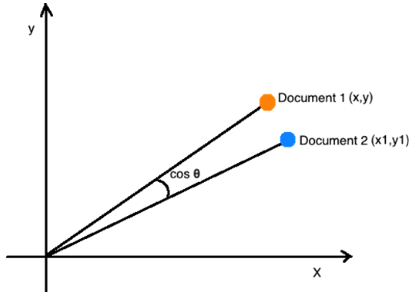
\includegraphics[scale=0.9]{cossine-similarity-1}
    \fonte{Ylber Januzaj e Artan Luma \textit{et al} (2022)}
    \label{fig:cossine_similarity_1}
\end{figure}

\begin{figure}[H]
    \caption{Documentos ortogonais no espaço vetorial}
    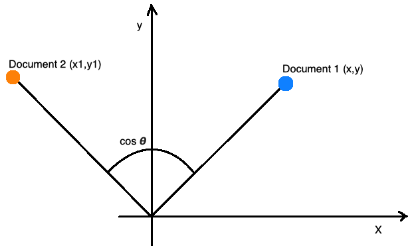
\includegraphics[scale=0.9]{cossine-similarity-2}
    \fonte{Ylber Januzaj e Artan Luma \textit{et al} (2022)}
    \label{fig:cossine_similarity_2}
\end{figure}

\begin{figure}[H]
    \caption{Documentos opostos no espaço vetorial}
    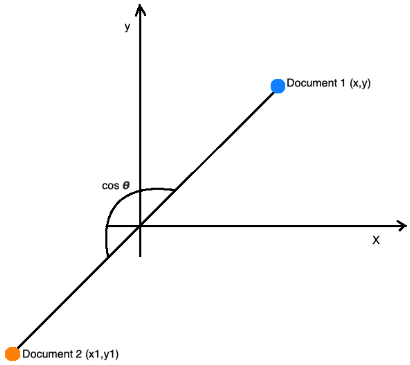
\includegraphics[scale=0.9]{cossine-similarity-3}
    \fonte{Ylber Januzaj e Artan Luma \textit{et al} (2022)}
    \label{fig:cossine_similarity_3}
\end{figure}

A implementação do método retorna um valor entre -1 e 1, onde valores negativos representam contradição entre os documentos, valor zero (vetores ortogonais) indicam não similaridade e valores positivos representam similaridade entre os documentos.

A partir da palavras-chave de cada laborátorio e do texto de uma demanda, calcula-se a pontuação de cada laboratório em relação a demanda seguindo a equação \ref{eq:score_equation}.

\begin{equation}
    \label{eq:score_equation}
    score =
    \begin{cases}
        \frac{\sum_{i=1}^{|k|} w_i \cdot \text{sim}\big(\text{embed}(d), \text{embed}(k_i)\big)}{|k|}, & \text{se } |k| > 0 \\
        0,                                                                                             & \text{se } |k| = 0
    \end{cases}
\end{equation}

Onde,

\begin{align*}                                                                                 \\
    d                & : \text{Texto da demanda}                          \\
    L                & : \text{Conjunto de laboratórios}                    \\
    l                & : \text{Um laboratório específico em } L                                  \\
    k                & : \text{Conjunto de palavras-chave do laboratório } l \\
    k_i              & : \text{Uma palavra-chave específica em } k                               \\
    w_i              & : \text{Peso associado à palavra-chave } k_i                              \\
    \text{embed}(x)  & : \text{Embedding gerado pelo modelo para o texto } x                     \\
    \text{sim}(a, b) & : \text{Similaridade entre os embeddings } a \text{ e } b                 \\
    S_l              & : \text{Score calculado para o laboratório } l
\end{align*}

\subsection{Marcação de Parte de Fala}\label{subsec:pos_tagging}

O modelo \gls{bert} requer um maior número de configurações para que possa ser utilizado de forma eficiente. Uma da configurações necessárias para sua utilização é marcação das partes de fala.

\gls{pos} representa a estrutura sintática das palavras em uma linguaguem, como por exemplo para o português brasileiro, tem-se o substantivo, adjetivo, artigo, numeral, pronome, verbo, advérbio, preposição, conjunção e interjeição. A marcação de partes de fala é uma das técnicas utilizadas para identificar e classificar as palavras de um texto de acordo com sua função gramatical, e serve o propósito de promover a desambiguação de palavras bem como auxiliar no entendimento da estrutura sintática \cite{JurafskyMartin2024}.

Sem a implementação da marcação de partes de fala, o desempenho do modelo na extração de contexto pode ser prejudicado a depender da linguagem do conjunto de dados, pois por padrão, o \gls{bert} é configurado e treinado para a língua inglesa. Existem duas formas de se implementar essa marcação, a primeira e mais simples é a utilização de expressões regulares, onde a estrutura de marcação é determinada por padrões presentes na expressão. A segunda forma, e a escolhida para este projeto, é automatizar o processo, cuja implementação pode ser vista na seção \ref{sec:implementacao}.